\documentclass{article}

\usepackage[utf8]{inputenc}
\usepackage[T1]{fontenc}
\usepackage[a4paper,margin=1in]{geometry}
\usepackage{amsmath}
\usepackage{booktabs}
\usepackage{natbib}
\usepackage{hyperref}
\usepackage{tabularx}
\usepackage{array}
\usepackage{pgfplots}
\usepackage{tikz}
\usepackage{xcolor}
\usepackage{siunitx}
\usepackage{cleveref}

\pgfplotsset{
    compat=1.18,
    my_style/.style={
        width=0.9\textwidth,
        axis lines=left,
        grid=major,
        grid style={dashed, gray!50},
        legend style={draw=none, fill=none, at={(0.5,-0.2)}, anchor=north}
    }
}

\title{Competitive Dynamics of Tesla and BYD in China's Electric Vehicle Market (2020--2024)}
\author{Market Data, Trends, Competitive Analysis, and Policy Synthesis}
\date{\today}

\begin{document}

\maketitle

\begin{abstract}
From 2020 to 2024, China's electric vehicle (EV) market experienced unprecedented growth, becoming the largest globally and accounting for over 60\% of global EV sales by 2024. This report provides a comprehensive analysis of the competitive dynamics between Tesla and BYD, the two dominant players in the Chinese EV sector. Drawing on quantitative sales data, market share trends, product and technology comparisons, financial performance, and the impact of government policies and infrastructure, we examine how BYD overtook Tesla in sales and market share, and how both companies adapted their strategies in response to evolving market conditions. The findings highlight the critical role of government support, technological innovation, and aggressive pricing in shaping the competitive landscape, offering insights for stakeholders and policymakers navigating the rapidly evolving Chinese EV market.
\end{abstract}

\section{Introduction}

China's electric vehicle (EV) market has undergone rapid transformation from 2020 to 2024, driven by robust government policies, technological innovation, and shifting consumer preferences. The Chinese government invested over \$230 billion in subsidies, tax breaks, and infrastructure development from 2009 through 2023, fostering a robust domestic EV industry and making China the world's largest EV market by volume \citep{techreview2023,csis2024}. Tesla entered the Chinese market in 2020 with its Shanghai Gigafactory, quickly becoming a major player due to local production and strong brand appeal. Meanwhile, BYD, a domestic manufacturer with roots in battery production, leveraged government support and vertical integration to expand aggressively. By 2024, BYD had surpassed Tesla in total EV sales in China, reflecting a broader trend of domestic brands gaining dominance in the new energy vehicle (NEV) market \citep{sciencedirect2023,reuters2025}.

\section{Market Share and Sales Volume Trends}

\subsection{Annual Sales and Market Share}

\begin{table}[ht]
\centering
\caption{Tesla and BYD Sales and Market Share in China, 2020--2024}
\label{tab:sales_market_share}
\begin{tabularx}{\textwidth}{l S[table-format=7.0] S[table-format=2.1] S[table-format=7.0] S[table-format=2.1] S[table-format=8.0]}
\toprule
Year & {Tesla China Sales (Units)} & {Tesla Market Share (\%)} & {BYD China Sales (Units)} & {BYD Market Share (\%)} & {Total China NEV Sales (Units)} \\
\midrule
2020 & 160000 & 12.4 & 170000 & 12.9 & 1300000 \\
2023 & 700000 & 8.5 & 2800000 & 30.0 & 9000000 \\
2024 & 657000 & 6.1 & 4270000 & 34.5 & 12870000 \\
\bottomrule
\end{tabularx}
\end{table}

\begin{figure}[ht]
\centering
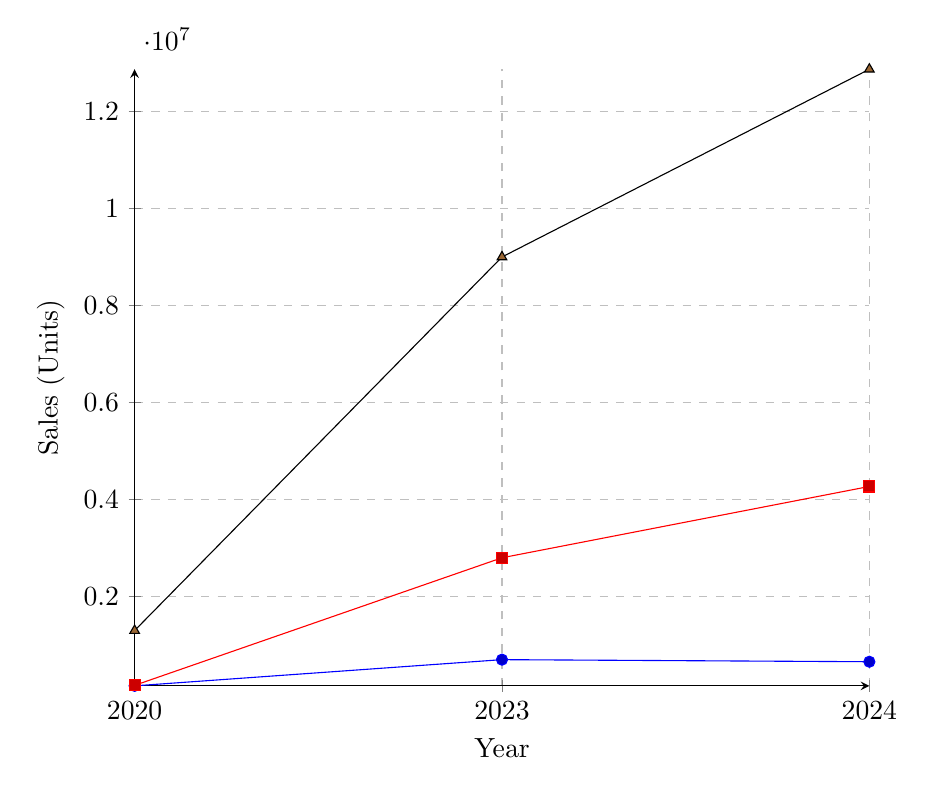
\begin{tikzpicture}
\begin{axis}[my_style, ylabel={Sales (Units)}, xlabel={Year}, xtick=data, symbolic x coords={2020,2023,2024}, legend columns=2, legend to name=legend1]
\addplot+[mark=*, color=blue] coordinates {(2020,160000) (2023,700000) (2024,657000)};
\addplot+[mark=square*, color=red] coordinates {(2020,170000) (2023,2800000) (2024,4270000)};
\addplot+[mark=triangle*, color=black] coordinates {(2020,1300000) (2023,9000000) (2024,12870000)};
\legend{Tesla, BYD, Total NEV}
\end{axis}
\end{tikzpicture}
\caption{Annual Sales of Tesla, BYD, and Total NEVs in China (2020--2024)}
\label{fig:sales_trend}
\end{figure}

\noindent
Tesla's China sales grew from an estimated 160,000 units in 2020 to 657,000 units in 2024, representing an 8.8\% increase in 2024 despite global delivery declines \citep{reuters2025,statista2024}. BYD's sales surged from approximately 170,000 units in 2020 to over 4.27 million in 2024, a growth rate exceeding 800\% over four years, driven by a diversified product portfolio including BEVs and PHEVs \citep{reuters2025,cnn2025}. BYD's market share in China's NEV market increased from 12.9\% in 2020 to over 32\% in 2024, while Tesla's share declined from 12.4\% to about 6.1\% in the same period \citep{statista2024,cnn2025}.

\subsection{Market Share Evolution}

\begin{figure}[ht]
\centering
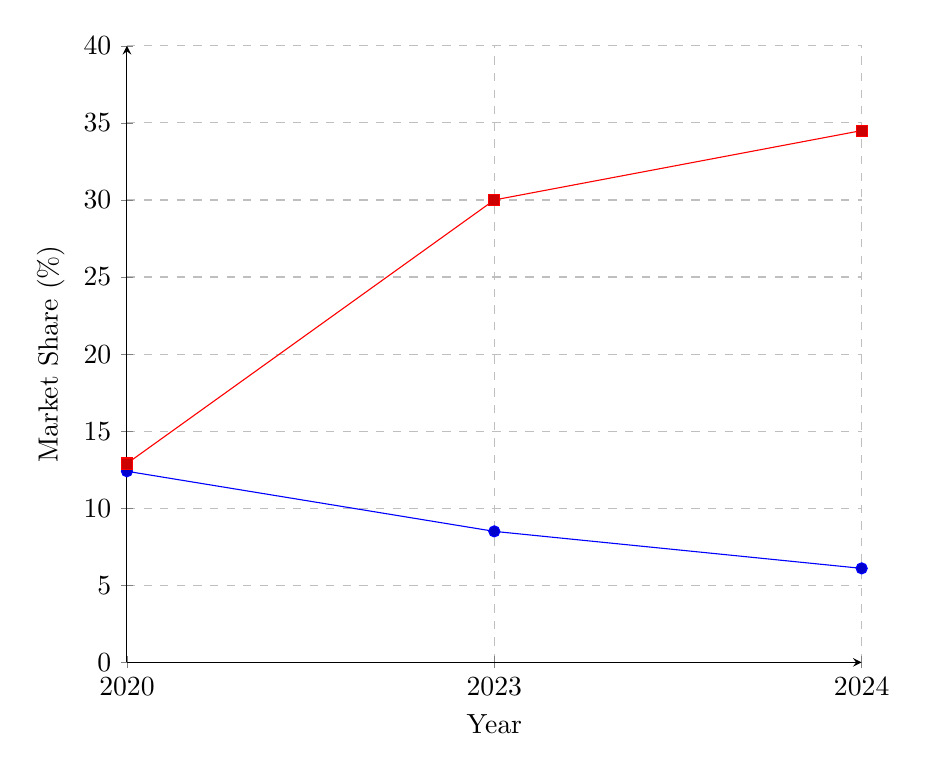
\begin{tikzpicture}
\begin{axis}[my_style, ylabel={Market Share (\%)}, xlabel={Year}, xtick=data, symbolic x coords={2020,2023,2024}, ymin=0, ymax=40, legend columns=2, legend to name=legend2]
\addplot+[mark=*, color=blue] coordinates {(2020,12.4) (2023,8.5) (2024,6.1)};
\addplot+[mark=square*, color=red] coordinates {(2020,12.9) (2023,30.0) (2024,34.5)};
\legend{Tesla, BYD}
\end{axis}
\end{tikzpicture}
\caption{Market Share of Tesla and BYD in China's NEV Market (2020--2024)}
\label{fig:market_share}
\end{figure}

\section{Product Portfolio and Technology Comparison}

\begin{table}[ht]
\centering
\caption{Product and Technology Comparison: Tesla vs. BYD (2024)}
\label{tab:product_tech}
\begin{tabularx}{\textwidth}{l X X}
\toprule
Feature & Tesla & BYD \\
\midrule
Product Range & Primarily BEVs: Model 3, Model Y, S, X & BEVs and PHEVs across multiple segments \\
Battery Technology & 4680 cylindrical cells, external suppliers & Blade LFP battery, in-house production \\
Charging Speed & 270 km in 15 minutes (Supercharger) & 400 km in 5 minutes (10C Blade battery) \\
Autonomy & Full Self-Driving (FSD) pending China approval & ``God's Eye'' ADAS standard on most models \\
Pricing Strategy & Premium pricing, recent discounts & Aggressive price cuts (10--34\%), broad affordability \\
Manufacturing Locations & Shanghai Gigafactory, US, Germany, Mexico & China (multiple plants), expanding overseas \\
\bottomrule
\end{tabularx}
\end{table}

BYD's Blade battery technology offers ultra-fast charging, adding 400 km range in 5 minutes, outperforming Tesla's Supercharger technology, which adds 270 km in 15 minutes \citep{cnn2025,investors2024}. Tesla's FSD remains unapproved in China, limiting its competitive edge in autonomous driving, whereas BYD offers advanced driver-assistance systems (ADAS) like ``God's Eye'' at no extra cost \citep{cnn2025}. BYD's product lineup spans from entry-level EVs priced below \$10,000 to premium models up to \$150,000, enabling broad market coverage. Tesla focuses on premium and mid-range segments, with Model 3 and Model Y as best sellers \citep{investors2024,aeternus2024}.

\section{Financial Performance}

\begin{table}[ht]
\centering
\caption{Financial Performance of Tesla and BYD (2024)}
\label{tab:financials}
\begin{tabularx}{\textwidth}{l S[table-format=7.1] S[table-format=7.1]}
\toprule
Metric & {Tesla (2024)} & {BYD (2024)} \\
\midrule
Revenue (USD) & 97700000000 & 107000000000 \\
Net Profit (USD) & 7100000000 & 5800000000 \\
Vehicle Sales (Global, Units) & 1790000 & 4270000 \\
Market Cap (May 2025, USD) & 1090000000000 & 162300000000 \\
R\&D Spending (\% Revenue) & 35.0 & 4.9 \\
\bottomrule
\end{tabularx}
\end{table}

\begin{figure}[ht]
\centering
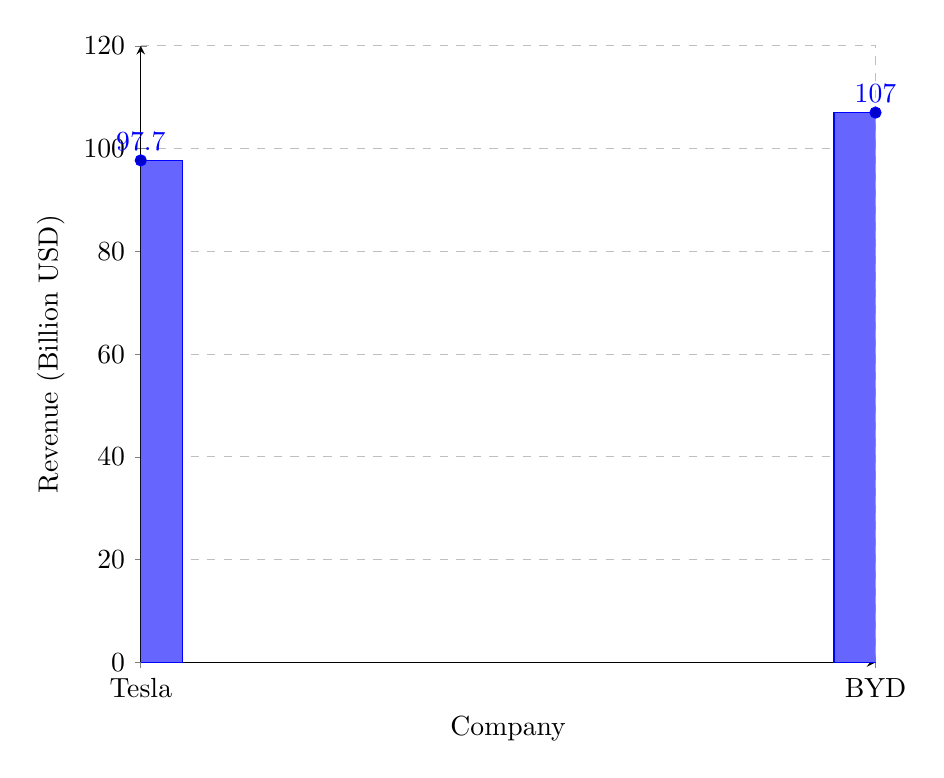
\begin{tikzpicture}
\begin{axis}[my_style, ylabel={Revenue (Billion USD)}, xlabel={Company}, symbolic x coords={Tesla,BYD}, xtick=data, ymin=0, ymax=120, nodes near coords, bar width=30pt]
\addplot+[ybar, fill=blue!60] coordinates {(Tesla,97.7) (BYD,107)};
\end{axis}
\end{tikzpicture}
\caption{2024 Revenue Comparison: Tesla vs. BYD}
\label{fig:revenue}
\end{figure}

BYD surpassed Tesla in revenue and total vehicle sales in 2024, driven by its diversified product portfolio and strong domestic market presence \citep{cnn2025,investors2024}. Tesla maintains a significantly higher market capitalization, reflecting investor confidence in its innovation and global brand, despite recent stock declines in 2025 \citep{investors2024}.

\section{Market Trends and Regulatory Environment}

China accounted for 70\% of global EV and hybrid sales in 2024, with NEVs surpassing 50\% of passenger car sales in March 2025 \citep{techinasia2025}. Government policies included purchase subsidies (phased out by end 2022), tax exemptions, license plate priority, and extensive charging infrastructure investments, which have been critical in driving EV adoption and supporting domestic manufacturers like BYD \citep{techreview2023,sciencedirect2024}. Charging infrastructure expanded rapidly, with over 12.8 million charging points by end 2024, a 49\% year-over-year increase, supporting consumer confidence and EV market growth \citep{argus2024}.

\begin{figure}[ht]
\centering
\begin{tikzpicture}
\begin{axis}[my_style, ylabel={Charging Points (Millions)}, xlabel={Year}, xtick=data, symbolic x coords={2020,2023,2024}, ymin=0, ymax=14, nodes near coords]
\addplot+[mark=*, color=green!60!black] coordinates {(2020,1.5) (2023,8.6) (2024,12.8)};
\end{axis}
\end{tikzpicture}
\caption{Growth of EV Charging Infrastructure in China (2020--2024) \citep{argus2024}}
\label{fig:charging}
\end{figure}

Intense price competition and a ``price war'' initiated by BYD in 2025 led to significant discounts (10--34\%) across multiple models, pressuring margins but boosting sales volume \citep{onglobal2025}.

\section{Competitive Positioning and Strategies}

\begin{table}[ht]
\centering
\caption{Competitive Strategies: Tesla vs. BYD}
\label{tab:strategies}
\begin{tabularx}{\textwidth}{l X X}
\toprule
Aspect & Tesla & BYD \\
\midrule
Pricing Strategy & Premium, with recent discounts & Aggressive price cuts, broad affordability \\
Marketing Approach & Minimal traditional advertising, brand strength, social media & Multi-channel marketing, sports sponsorships, dealer networks \\
Geographic Focus & Major urban centers, affluent consumers & Broad coverage including 2nd/3rd tier cities \\
Production Strategy & Localized Shanghai Gigafactory, global expansion & Vertical integration, multiple plants in China, expanding overseas \\
Innovation Focus & Battery tech (4680 cells), FSD software & Battery tech (Blade battery), fast charging, ADAS \\
\bottomrule
\end{tabularx}
\end{table}

Tesla relies on brand prestige, innovation, and localized production to maintain market share in premium segments, while BYD leverages vertical integration, cost leadership, and a diversified product range to dominate the mass market \citep{daxue2024,aeternus2024}. BYD's rapid model refresh cycles (average model age 1.6 years vs. Tesla's 5.4 years) and extensive product launches (40+ new models since 2020) contrast with Tesla's slower product updates, contributing to BYD's competitive advantage \citep{reuters2025}. BYD's international expansion includes plants in Thailand, Brazil, Hungary, and plans for Mexico and Europe, while Tesla faces challenges in Europe and China due to tariffs and competition \citep{investors2024,jato2024}.

\section{Comparative Analysis: 2024 Snapshot}

\begin{table}[ht]
\centering
\caption{Tesla vs. BYD in China: Key Metrics (2024)}
\label{tab:comparison}
\begin{tabularx}{\textwidth}{l X X}
\toprule
Metric/Aspect & Tesla (China, 2024) & BYD (China, 2024) \\
\midrule
Sales Volume (Units) & 657,000 & 4,270,000 \\
Market Share (\%) & 6.1 & 32--37 \\
Revenue (USD) & \$20.9 billion (China) & \$107 billion (total) \\
Product Range & BEVs only & BEVs + PHEVs \\
Average Price Range (USD) & \$38,000+ (Model 3 RWD base) & \$9,700--\$150,000 \\
Charging Speed & 270 km in 15 min (Supercharger) & 400 km in 5 min (Blade battery) \\
Autonomy & FSD pending China approval & Level 2+ ADAS standard, LiDAR on premium models \\
Production Capacity (Units) & $\sim$1.8 million globally & 4.3 million (2024) \\
R\&D Intensity (\% Revenue) & $\sim$35 & $\sim$4.9 \\
Marketing Strategy & Brand strength, minimal ads & Multi-channel, sports sponsorships \\
Geographic Penetration & Urban, affluent centers & Broad, including 2nd/3rd tier cities \\
\bottomrule
\end{tabularx}
\end{table}

This comparison highlights BYD's dominance in volume and market share, supported by a broad product portfolio and aggressive pricing, while Tesla leads in innovation, brand prestige, and premium market segments.

\section{Government Policy, Subsidies, and Infrastructure}

China's government has played a pivotal role in shaping the EV market through a combination of direct subsidies, tax incentives, infrastructure investment, and regulatory support. From 2009 to 2023, over \$230 billion was invested in the sector, supporting both domestic and foreign manufacturers \citep{csis2024,techreview2023}. Key policy measures included:

\begin{itemize}
    \item \textbf{Purchase subsidies:} Phased out by end 2022, but critical in early market expansion.
    \item \textbf{Tax exemptions and license plate priority:} Lowered barriers for consumers.
    \item \textbf{Charging infrastructure:} Over 12.8 million charging points by 2024, a 49\% YoY increase \citep{argus2024}.
    \item \textbf{Industrial policy:} Support for battery supply chains, local production, and export incentives.
\end{itemize}

These policies have enabled rapid innovation, cost reduction, and market penetration for domestic brands like BYD, while also supporting Tesla's localized production and sales growth \citep{techreview2023,sciencedirect2024,csis2024}.

\section{Conclusions and Future Outlook}

The period from 2020 to 2024 saw BYD emerge as the dominant EV manufacturer in China, surpassing Tesla in sales volume, market share, and revenue. BYD's success is underpinned by strong government support, vertical integration, aggressive pricing, rapid product development, and expanding international presence. Tesla, while maintaining a strong foothold in the premium segment and leading in technological innovation, faces increasing competitive pressure from BYD and other domestic manufacturers, especially as BYD's fast-charging technology and ADAS offerings gain traction \citep{cnn2025,investors2024,reuters2025}.

Looking ahead, China's EV market is expected to continue growing robustly, with NEVs projected to exceed 50\% of passenger car sales by 2025 \citep{techinasia2025}. BYD's expansion into international markets and continued innovation in battery and charging technologies position it well for sustained growth. Tesla's future success in China will depend on its ability to diversify its product lineup, reduce prices, and enhance local market adaptation amid intensifying competition and regulatory challenges \citep{techinasia2025,argus2024}.

Both companies face external challenges, including tariffs, geopolitical tensions, and evolving consumer preferences. The Chinese government's continued support for EV infrastructure and industrial policy will remain a critical factor shaping the competitive landscape. The ongoing price war initiated by BYD may pressure industry profitability but also accelerates consumer adoption and market penetration \citep{onglobal2025}.

\begin{quote}
``BYD's rapid innovation, aggressive pricing, and vertical integration have allowed it to dominate China and expand globally, while Tesla's slower adaptation and premium focus have led to market share erosion in China'' \citep{restofworld2025}.
\end{quote}

\section*{Acknowledgments}
This report synthesizes data and analysis from multiple authoritative sources to provide a detailed, accurate, and nuanced understanding of Tesla and BYD's competitive dynamics in the Chinese EV market from 2020 to 2024.

\bibliographystyle{unsrt}
\bibliography{references}

\begin{filecontents*}{references.bib}
@article{reuters2025,
  title={Tesla's China sales hit record high in 2024, bucking global decline},
  author={Reuters},
  year={2025},
  note={\url{https://www.reuters.com/business/autos-transportation/teslas-china-sales-rise-record-high-83000-december-2025-01-03}}
}
@article{cnn2025,
  title={Chinese EV titan BYD annual sales hit \$100 billion eclipsing rival Tesla},
  author={CNN},
  year={2025},
  note={\url{https://www.cnn.com/2025/03/25/cars/china-byd-annual-sales-pass-tesla-intl-hnk}}
}
@article{statista2024,
  title={China: Share of the new energy vehicle market by manufacturer},
  author={Statista},
  year={2024},
  note={\url{https://www.statista.com/statistics/1279346/new-energy-vehicle-chinese-market-shares-by-manufacturer}}
}
@article{investors2024,
  title={Tesla Vs. BYD As Of May 26: TSLA Has New Buy Point; BYD Launches Price War},
  author={Investors.com},
  year={2024},
  note={\url{https://www.investors.com/news/tesla-vs-byd-ev-sales-robotaxis}}
}
@article{aeternus2024,
  title={The Journey to the Top: BYD’s Marketing Strategy},
  author={Aeternus},
  year={2024},
  note={\url{https://www.aeternus.rs/the-journey-to-the-top-byds-marketing-strategy}}
}
@article{techreview2023,
  title={How did China come to dominate the world of electric cars?},
  author={Technology Review},
  year={2023},
  note={\url{https://www.technologyreview.com/2023/02/21/1068880/how-did-china-dominate-electric-cars-policy}}
}
@article{csis2024,
  title={The Chinese EV Dilemma: Subsidized Yet Striking | Trustee China Hand | CSIS},
  author={CSIS},
  year={2024},
  note={\url{https://www.csis.org/blogs/trustee-china-hand/chinese-ev-dilemma-subsidized-yet-striking}}
}
@article{sciencedirect2023,
  title={Competition and welfare effects of introducing new products into the new energy vehicle market: Empirical evidence from Tesla’s entry into the Chinese market},
  author={ScienceDirect},
  year={2023},
  note={\url{https://www.sciencedirect.com/science/article/abs/pii/S0965856423001507}}
}
@article{reuters2025,
  title={How China's new auto giants left GM, VW and Tesla in the dust},
  author={Reuters},
  year={2025},
  note={\url{https://www.reuters.com/investigations/how-chinas-new-auto-giants-left-gm-vw-tesla-dust-2025-07-03}}
}
@article{techinasia2025,
  title={China sets record with new EVs surpassing 50\% market share},
  author={Tech in Asia},
  year={2025},
  note={\url{https://www.techinasia.com/news/china-sets-record-with-new-evs-surpassing-50-market-share}}
}
@article{sciencedirect2024,
  title={Policy incentives and electric vehicle adoption in China: From a perspective of policy mixes},
  author={ScienceDirect},
  year={2024},
  note={\url{https://www.sciencedirect.com/science/article/pii/S0965856424002830}}
}
@article{argus2024,
  title={China expands EV charging infrastructure in 2024 - Argus Media},
  author={Argus Media},
  year={2024},
  note={\url{https://www.argusmedia.com/en/news-and-insights/latest-market-news/2650730-china-expands-ev-charging-infrastructure-in-2024}}
}
@article{onglobal2025,
  title={BYD NEEDS A NEW PRICE STRATEGY - On Global Leadership},
  author={On Global Leadership},
  year={2025},
  note={\url{https://ongloballeadership.com/f/byd-needs-a-new-price-strategy?ref=heysummit&blogcategory=Local+Government}}
}
@article{daxue2024,
  title={BYD’s electric dream: From humble beginning to a global EV powerhouse},
  author={Daxue Consulting},
  year={2024},
  note={\url{https://daxueconsulting.com/byd-electric-vehicles-market-in-china}}
}
@article{jato2024,
  title={BYD outsells Tesla in Europe for the first time as registrations surge in April},
  author={JATO},
  year={2024},
  note={\url{https://www.jato.com/resources/media-and-press-releases/byd-outsells-tesla-in-europe-for-the-first-time-as-registrations-surge-in-april}}
}
@article{restofworld2025,
  title={How Tesla blew its lead},
  author={Rest of World},
  year={2025},
  note={\url{https://restofworld.org/2025/tesla-loses-ground-chinese-ev-dominate-global-markets}}
}
\end{filecontents*}

\end{document}